\begin{frame}
\section{}
We saw an implementation of MLP in numpy and PyTorch. You may have noticed that the weights are initialized randomly. What happens if we we set all weights and biases to 0

Assume we are using ReLU activation

\begin{enumerate}[label=(\Alph*)]
\item Weights do not change while training    % Ans
\item No problem: the model will converge nicely
\item Overfitting issue
\item Underfitting issue
\item None of these  % None
\end{enumerate}
\end{frame}

\begin{frame}
\section{}
We saw this implementation of MLP model in PyTorch:

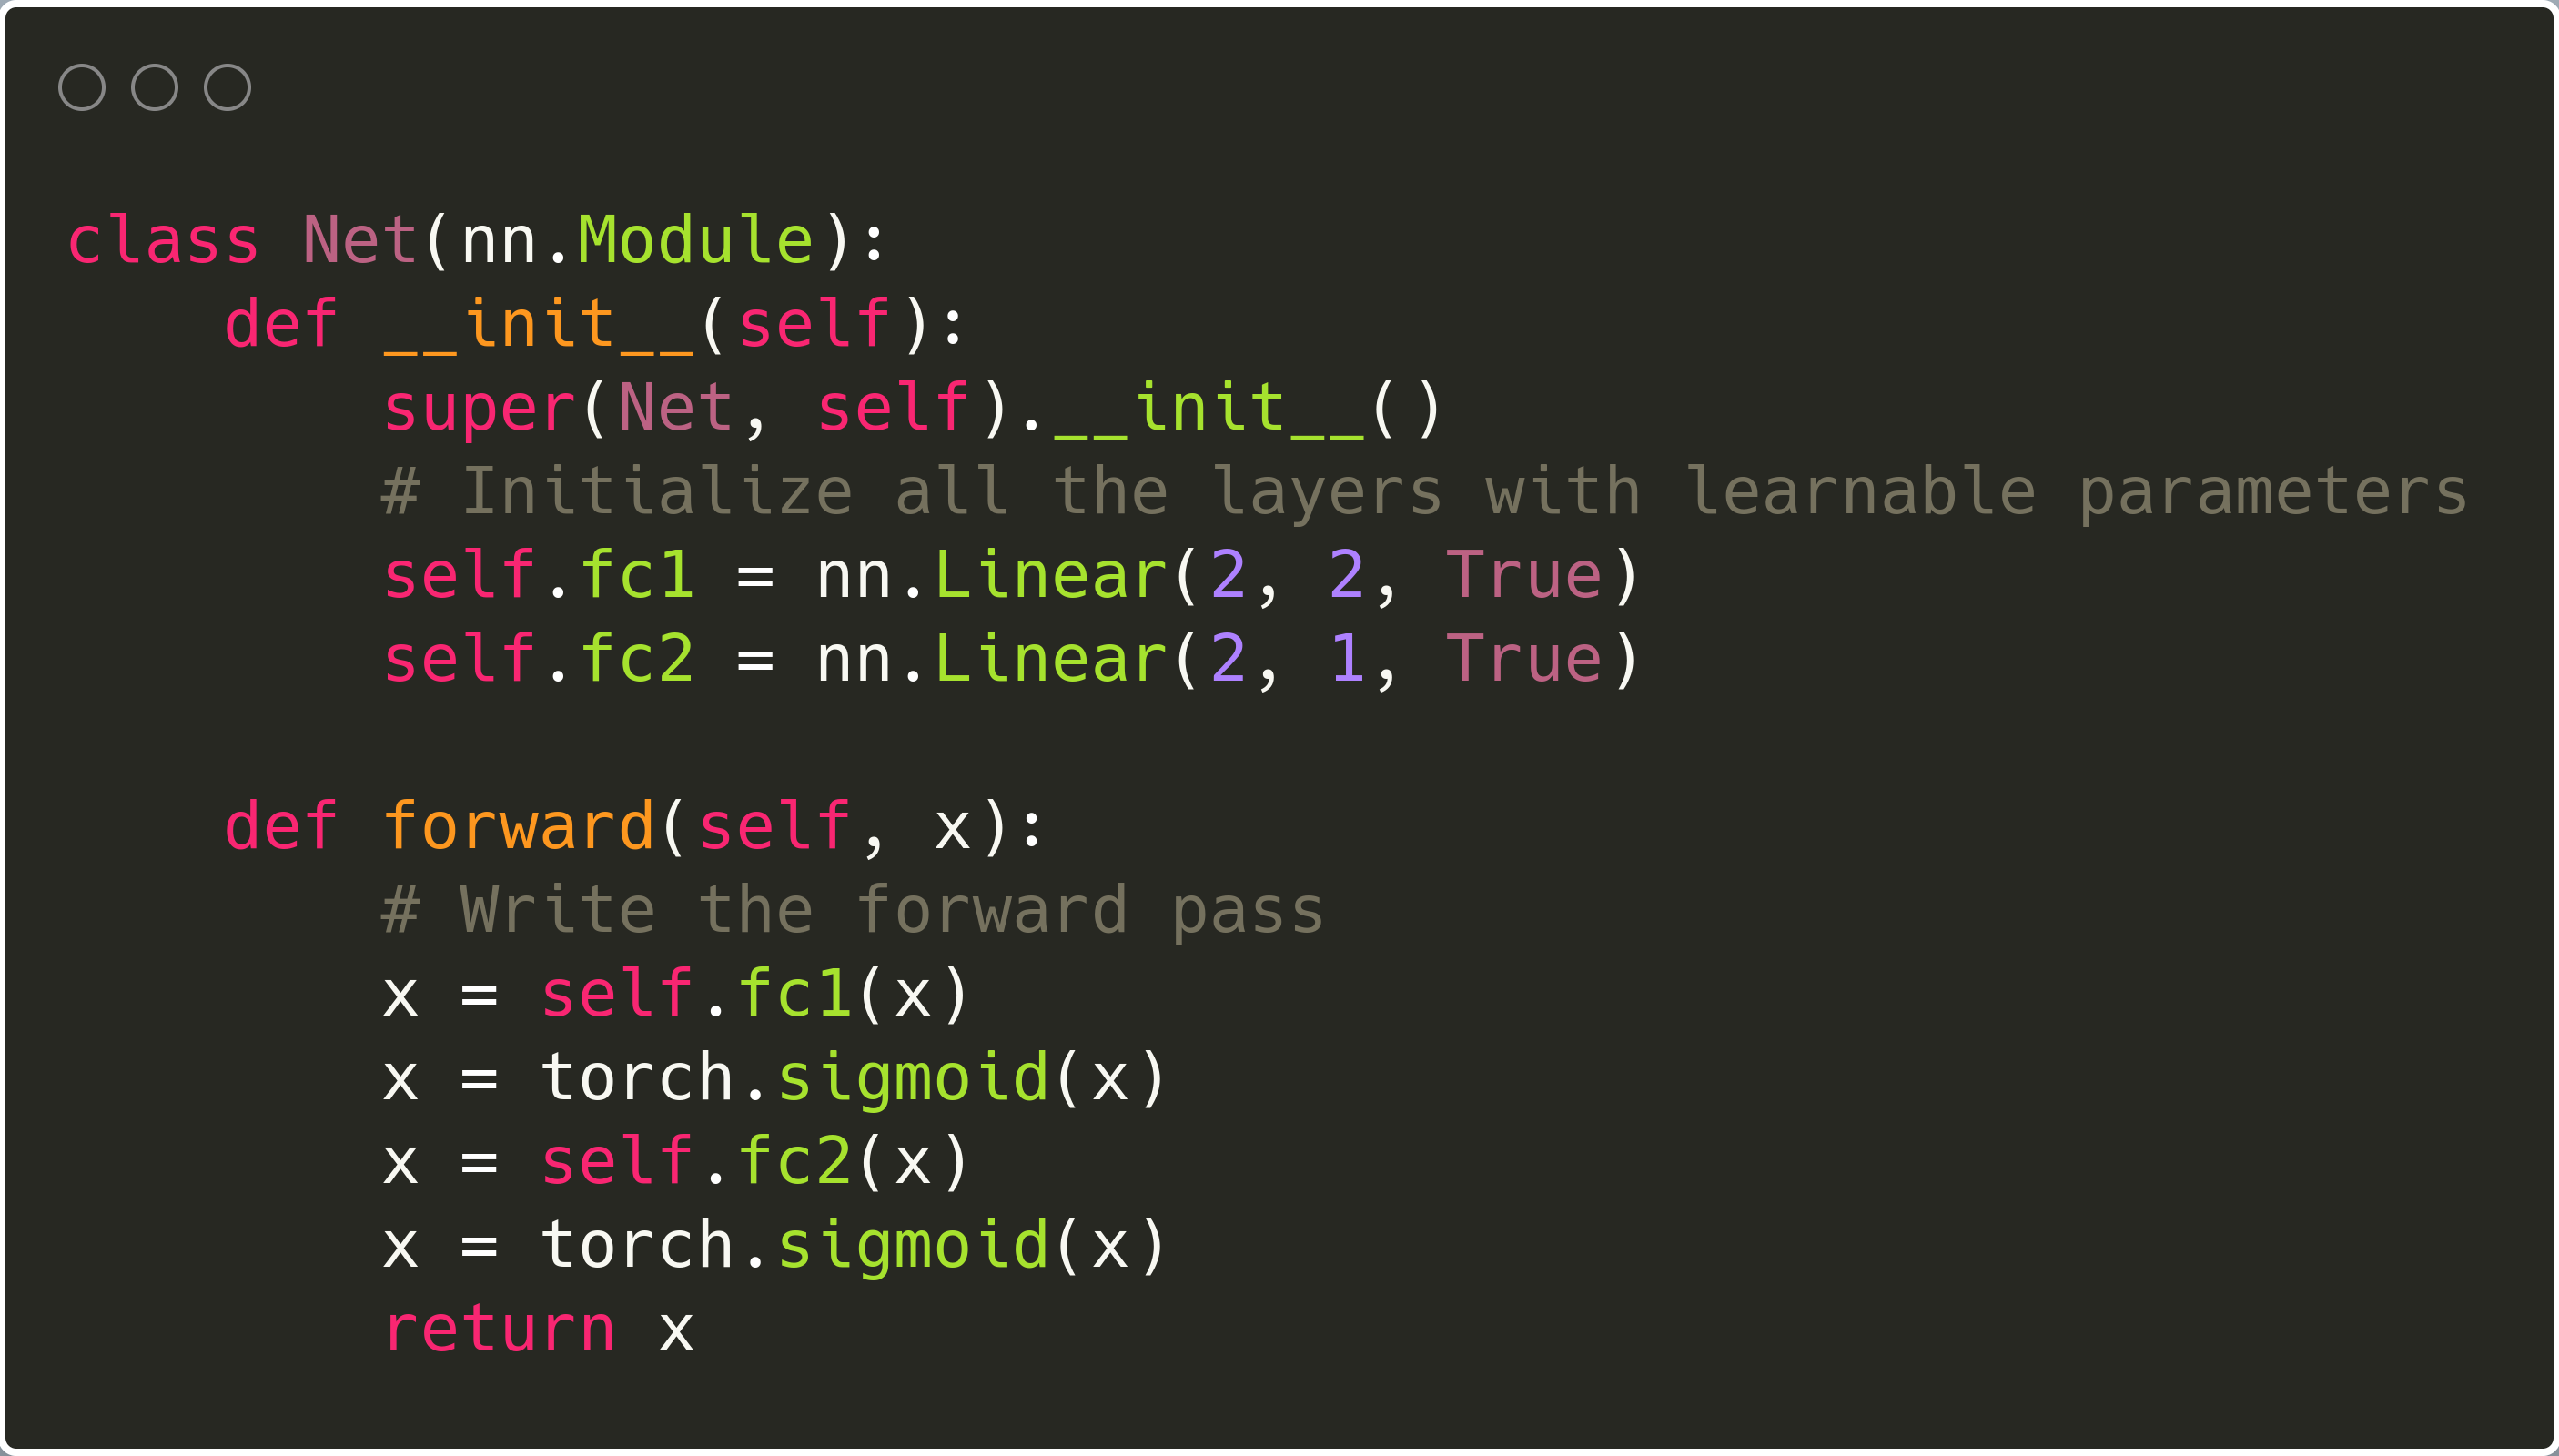
\includegraphics[scale=0.1]{images/q31_2.png}

The output of this model is
\begin{enumerate}[label=(\Alph*)]
\item Always greater than zero    % Ans
\item Always less than one   % Ans
\item Can be negative as well as positive
\item Always zero
\item None of these   % None
\end{enumerate}
\end{frame}

\begin{frame}
\section{}
We saw this implementation of MLP in PyTorch:

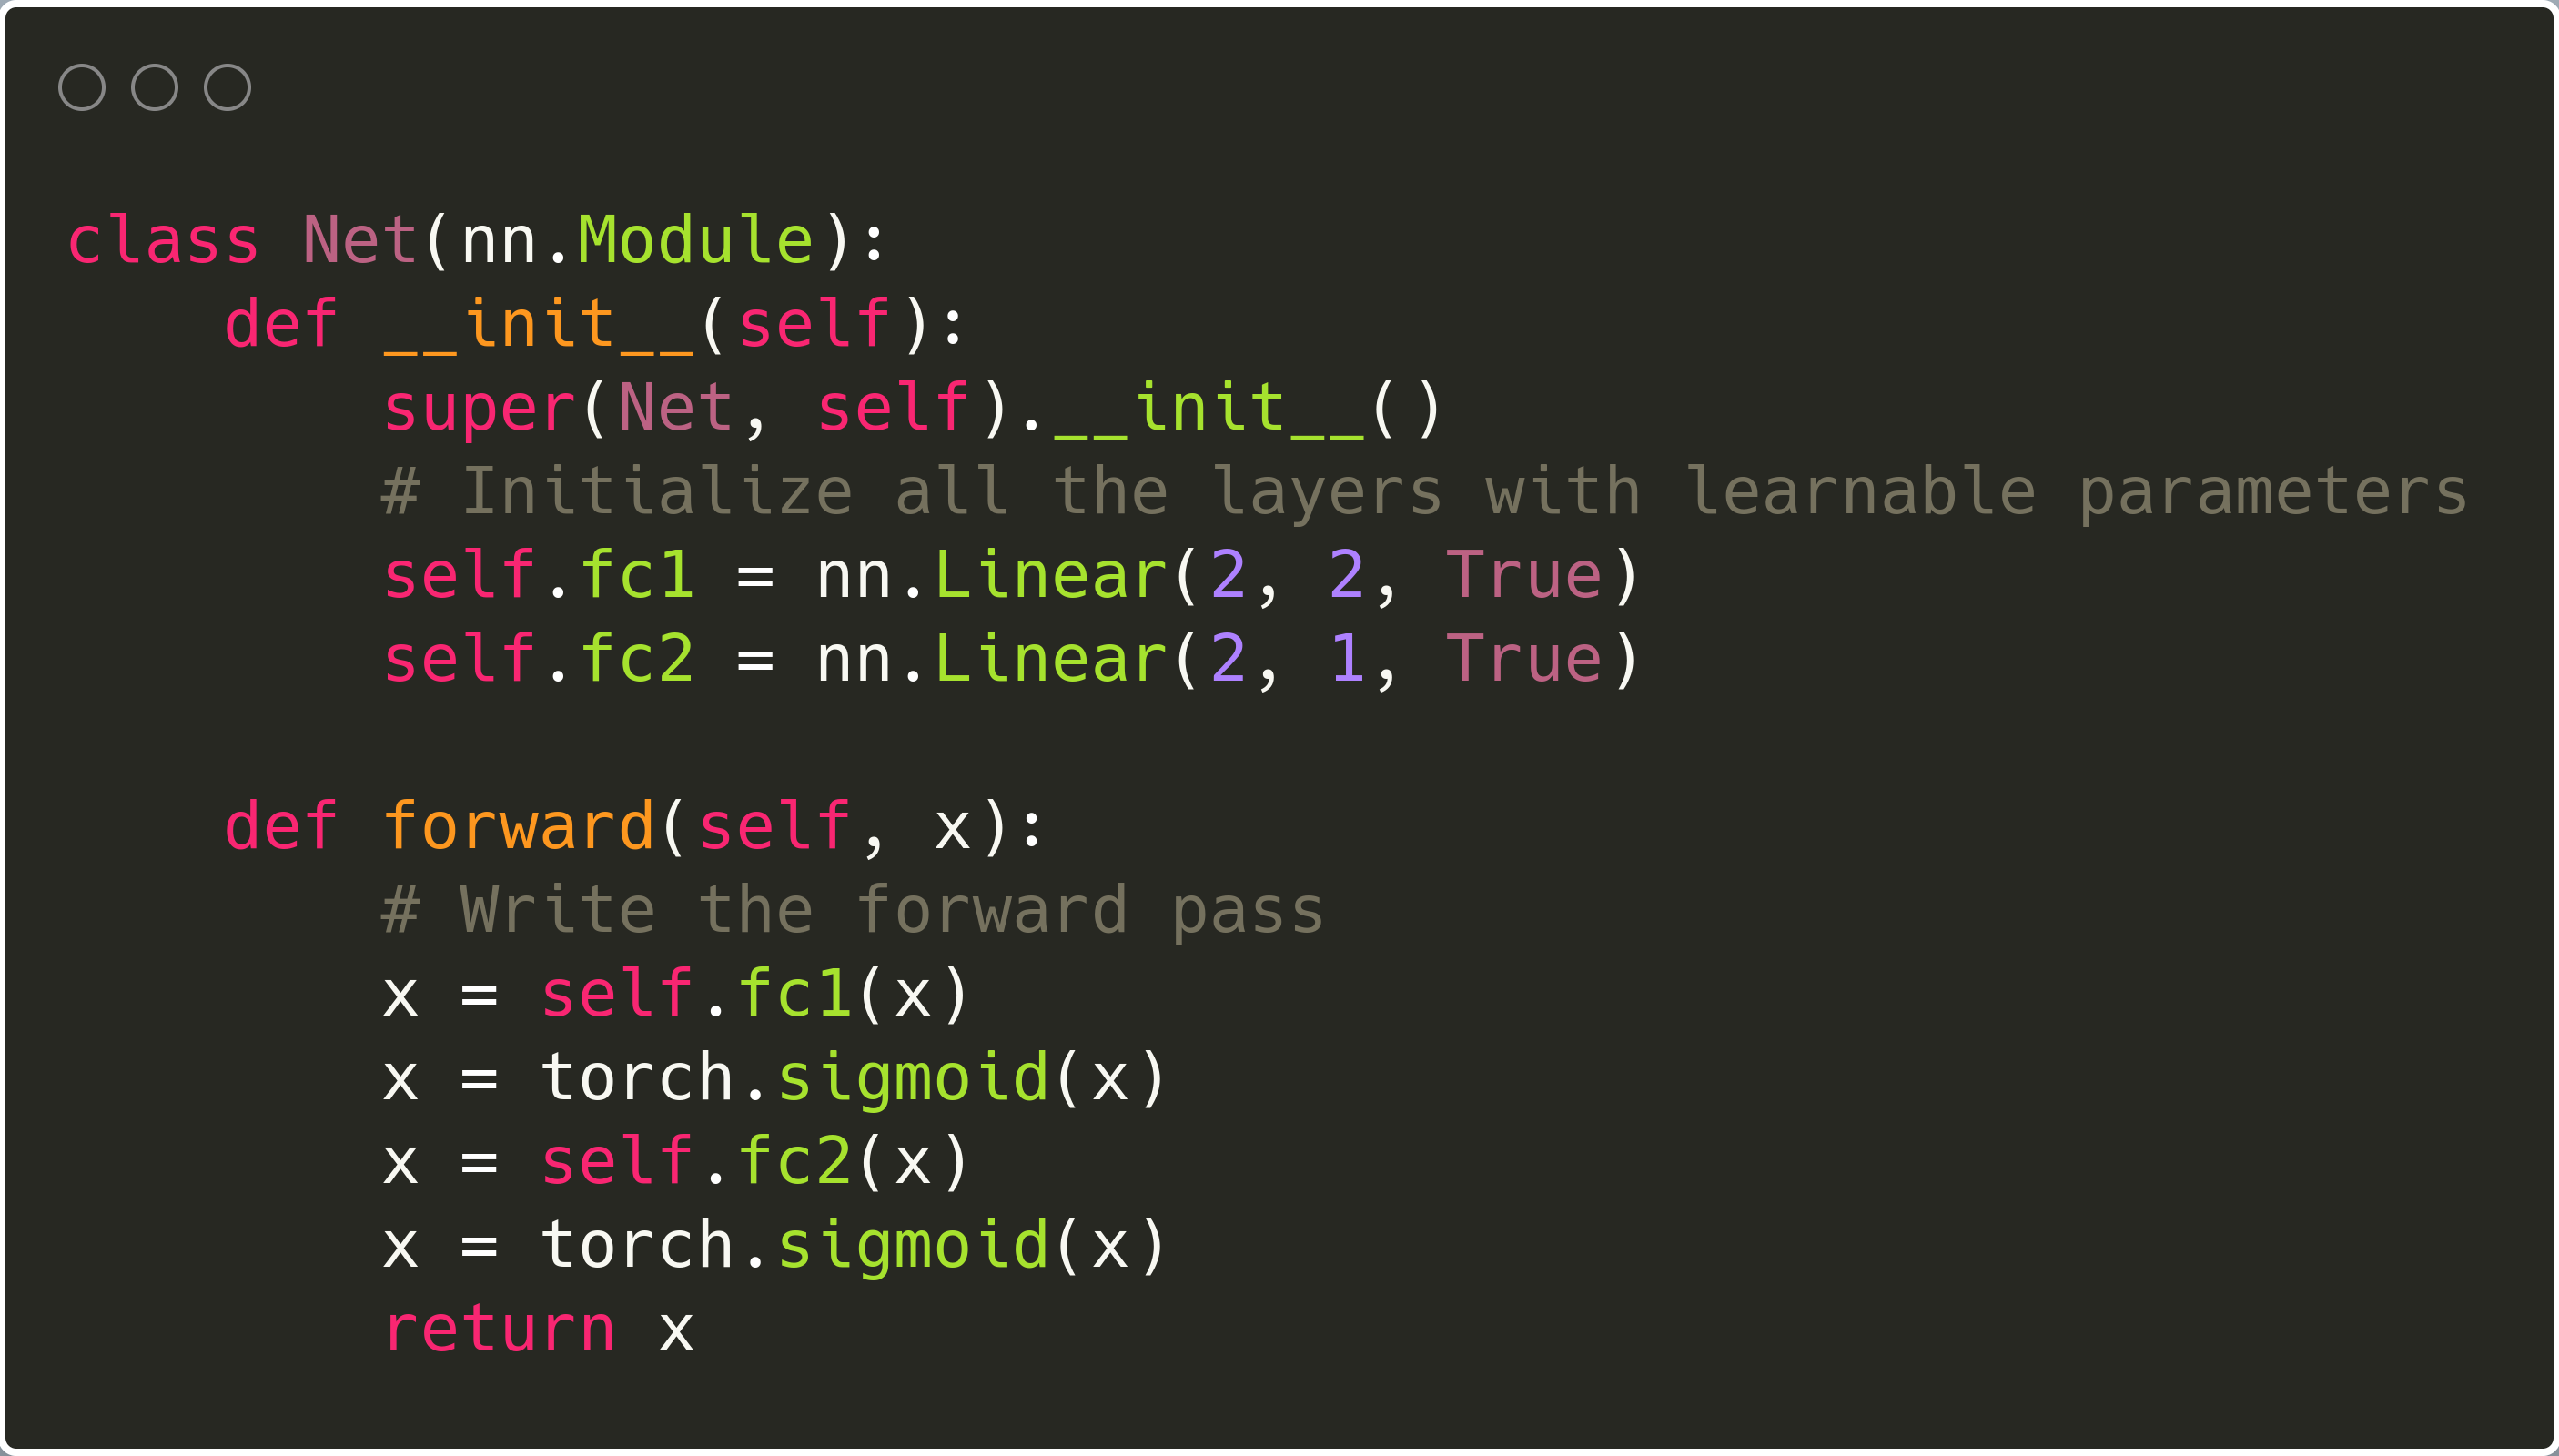
\includegraphics[scale=0.1]{images/q31_2.png}

What happens if we remove the 2 lines with code x=torch.sigmoid(x) in the forward function

Assume that we are working with the XOR data as given in the notebook shared.

\begin{enumerate}[label=(\Alph*)]
\item Syntax error
\item Math error
\item Model becomes Single layer perceptron   % Ans
\item Model remains multi layer perceptron
\item None of these    % None
\end{enumerate}
\end{frame}


\begin{frame}
\section{}
We saw the implementation of MLP in PyTorch with XOR data. What happens if we add 10 more hidden layers with 100 weights each with non-linear activation and train the model till loss is minimized.
\begin{enumerate}[label=(\Alph*)]
\item Results in the same decision boundary
\item Results in a different decision boundary but still able to classify all 4 samples correctly.    % Ans
\item Can not classify all 4 samples correctly.
\item None of these  % None
\end{enumerate}
\end{frame}



\begin{frame}
\section{}
Suppose instead of XOR data, we now want to work on NAND data. Model 1 is a MLP with a hidden layer with 2 neurons as we saw. Model 2 is a SLP.
\begin{enumerate}[label=(\Alph*)]
\item Model 1 can classify all 4 samples correctly but not model 2
\item Model 2 can classify all 4 samples correctly but not model 1
\item Both model 1 and model 2 can classify all 4 samples correctly.     % Ans
\item Neither model 1 nor model 2 can classify all 4 samples correctly.
\item None of these  % None
\end{enumerate}
\end{frame}
